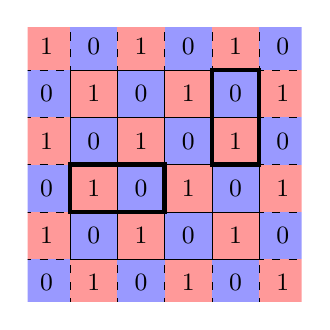
\begin{tikzpicture}[scale=.6,font=\small,anchor=center]

	\begin{scope}
		\clip (-0.9,-0.9) rectangle +(5.8,5.8);	
		
		\foreach \y in {-2,0,2,4}
		{
			\foreach \x in {-2,0,2,4}
			{				
				\fill[blue!40]	 	(\x+0,\y+0) rectangle +(1,1);
				\fill[red!40]	 	(\x+0,\y+1) rectangle +(1,1);
				\fill[red!40]		(\x+1,\y+0) rectangle +(1,1);
				\fill[blue!40] 		(\x+1,\y+1) rectangle +(1,1);
				
				\draw	(\x+0.5,\y+0.5) node{$0$};
				\draw	(\x+0.5,\y+1.5) node{$1$};
				\draw	(\x+1.5,\y+0.5) node{$1$};
				\draw	(\x+1.5,\y+1.5) node{$0$};
			}
		}
		
		\draw[help lines, black]		(0,0) grid +(4,4);
		\draw[help lines, dashed, black]		(-1,-1) grid +(6,6);
		
		\draw[ultra thick, black]	(0,1) rectangle +(2,1);
		\draw[ultra thick, black]	(3,2) rectangle +(1,2);
		
	\end{scope}	

\end{tikzpicture}